\section{O sistema de coordenadas polares}
\label{sec:coordpolar}

Um \emph{sistema de coordenadas} serve para representar a \emph{localização}
de um ponto no plano, através de um \emph{par ordenado} de números
chamados de \emph{coordenadas}.

Usualmente, quando representamos um ponto no plano, estamos nos
referindo ao \textbf{sistema de coordenadas retangulares}
(cartesianas), que são distâncias orientadas a partir de dois eixos
perpendiculares.

No sistema de coordenadas retangulares a localização de um ponto
$P$ é dada por

\begin{equation}
  P = (a, b)
\end{equation}

\noindent onde $a$ é a projeção de $P$ no eixo $x$, e $b$ é a projeção de $P$ no
eixo $y$.

Entretanto, para descrever curvas que exibem uma espécie de ``afinidade especial
por um ponto de origem'', como um círculo ou a trajetória de um
planeta ao longo de sua órbita, é melhor utilizar um outro sistema de
coordenadas, o sistema de coordenadas polares.

No \textbf{sistema de coordenadas polares} uma curva é descrita como a
trajetória de um ponto móvel cuja posição é especificada pela sua
\emph{direção a partir da origem} e pela sua \emph{distância até a
  origem}. Assim, qualquer ponto é localizado através de sua
\emph{direção} e sua \emph{distância} em relação à origem
(figura~\ref{fig:eixopolar}):

\begin{figure}[H]
  \begin{center}
    \caption{O eixo polar}
    \label{fig:eixopolar}
    \fbox{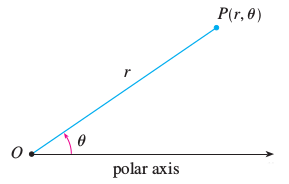
\includegraphics[scale=0.85]{imagens/int10.png}}\\
    \footnotesize{James Stewart: \emph{Cálculo} (8ª ed.,\ vol.\ 2,
      pg.\ 596)}
  \end{center}
\end{figure}

A direção é dada pelo ângulo $\theta$ em relação ao eixo polar
(geralmente em \emph{radianos}), e a distância $r$ é a distância
direta da origem até o ponto.

Esses dois números, $r$ e $\theta$,
são o par ordenado que formam as \emph{coordenadas polares} da
localização de um ponto no plano.

Por convenção, o par de coordenadas
polares é escrito primeiro informando-se a distância, e depois o ângulo:

\begin{equation}
  P = (r, \theta)
\end{equation}

Note o seguinte (figura~\ref{fig:caracteristicaspolar}):

\begin{itemize}[noitemsep]
  \item Esqueça o pensamento cartesiano de esquerda/direita (eixo $x$)
    e acima/abaixo (eixo $y$).
  \item Pense em termos de \emph{ao redor} e de
    \emph{distância} em relação ao \emph{polo}, a origem.
  \item $r = 0$ especifica a origem, independente de $\theta$.
  \item Cada ponto tem muitos pares de coordenadas polares, pois
    qualquer múltiplo de $2\pi$ adicionado ou subtraído de $\theta$
    faz uma ``volta completa'' na direção, parando no mesmo ponto.
  \item Cada coordenada polar define exatamente um ponto.
  \item Se aumentarmos $\theta$ por $\pi$, estamos na mesma ``reta''
    mas na direção contrária:
    \begin{equation}
      (r, \theta + \pi) = (-r, \theta)
    \end{equation}
\end{itemize}

\begin{figure}[H]
  \begin{center}
    \caption{Particularidades das coordenadas polares}
    \label{fig:caracteristicaspolar}
    \fbox{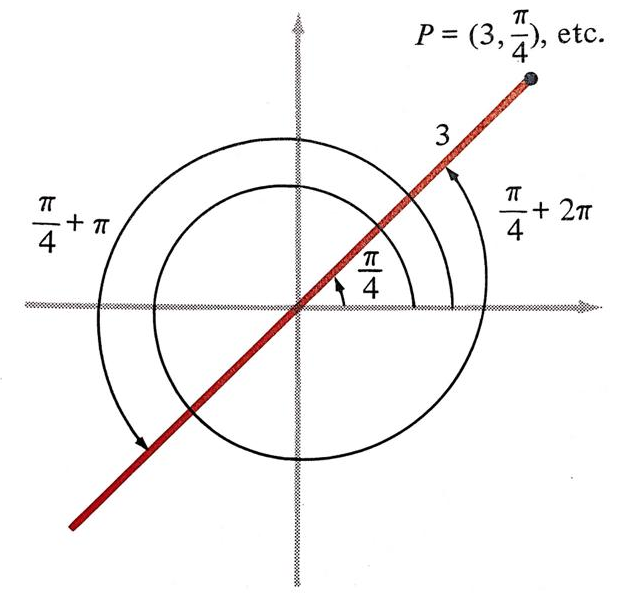
\includegraphics[scale=0.3]{imagens/int11.png}}\\
    \footnotesize{George Simmons: \emph{Calculus with Analytic
            Geometry} (2ª ed.,\ pg.\ 560)}
  \end{center}
\end{figure}

Uma representação interessante do sistema de coordenadas polares e de
como os pontos são localizados é
exibida nas figuras~\ref{fig:sistpolar} e \ref{fig:sistpolar2}, abaixo:

\begin{figure}[H]
  \begin{center}
    \caption{O sistema de coordenadas polares}
    \label{fig:sistpolar}
    \fbox{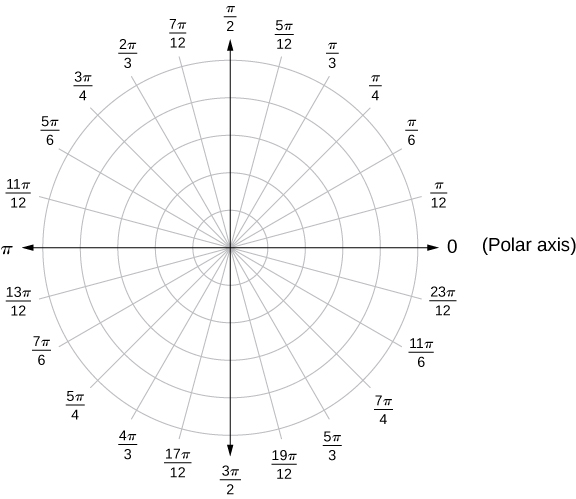
\includegraphics[scale=0.8]{imagens/int16.jpg}}\\
    \footnotesize{Gilbert Strang \& Edwin Herman: \emph{Calculus}
          (ed.\ online, 2017, vol.\ 2, pg.\ 645)}
  \end{center}
\end{figure}

\begin{figure}[H]
   \begin{center}
     \caption{Os pontos estão ao redor da origem}
     \label{fig:sistpolar2}
     \fbox{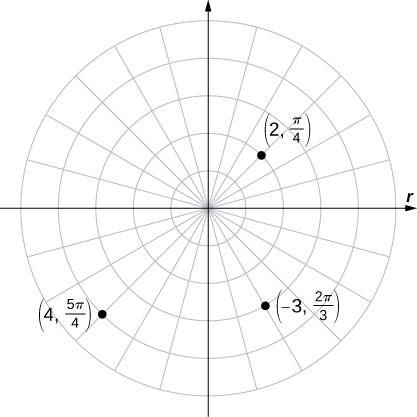
\includegraphics[scale=0.9]{imagens/int17.jpg}}\\
     \footnotesize{Gilbert Strang \& Edwin Herman: \emph{Calculus}
          (ed.\ online, 2017, vol.\ 2, pg.\ 646)}
     \end{center}
\end{figure}



\subsection{Equações e curvas polares}
\label{sec:coordpolar-eqcurv}

Para ilustrar de modo cristalino como uma mesma função pode ser
entendida de forma diferente dependendo do sistema de coordenadas
utilizado (retangular ou polar), considere a seguinte função: $r =
\cos(2\theta)$. Se essa função for plotada em coordenadas
retangulares, será uma onda; se for plotada em coordenadas polares
será uma rosa (figura~\ref{fig:mesmafuncdifview}):

\begin{figure}[H]
    \begin{center}
      \caption{Mesma função, dois pontos de vista}
      \label{fig:mesmafuncdifview}
      \fbox{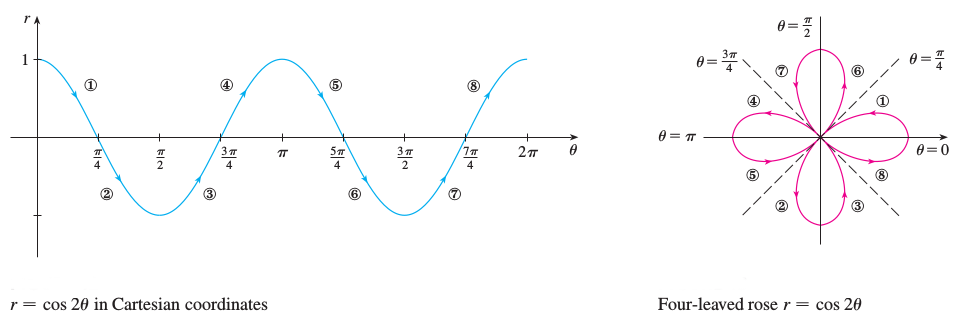
\includegraphics[scale=0.45]{imagens/int15.png}}\\
      \footnotesize{James Stewart: \emph{Cálculo} (8ª ed.,\ vol.\ 2, pg.\ 600)}
    \end{center}
\end{figure}

O gráfico de uma equação polar $r = f(\theta)$ ou, mais genericamente,
$F(r,\theta)=0$, consiste de todos os pontos $P$ que têm \emph{pelo
  menos uma} representação $(r, \theta)$ cujas coordenadas satisfaçam
a equação polar. Isso faz com que as equações polares, quando
plotadas, assumam formas belas e inusitadas (ver figuras:
\ref{fig:belo1}, \ref{fig:belo2}, \ref{fig:belo3}, \ref{fig:belo4},
\ref{fig:belo5}, \ref{fig:belo6}, \ref{fig:belo7}).

\begin{figure}[H]
  \begin{center}
    \caption{A beleza polar: espiral}
    \label{fig:belo1}
    \fbox{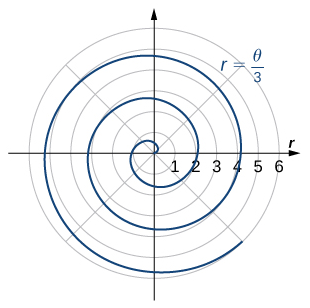
\includegraphics[scale=0.5]{imagens/int18.png}}\\
    \footnotesize{Gilbert Strang \& Edwin Herman: \emph{Calculus}
      (ed.\ online, 2017, vol.\ 2, pg.\ 651)}
  \end{center}
\end{figure}

\begin{figure}[H]
  \begin{center}
    \caption{A beleza polar: cardióde}
    \label{fig:belo2}
    \fbox{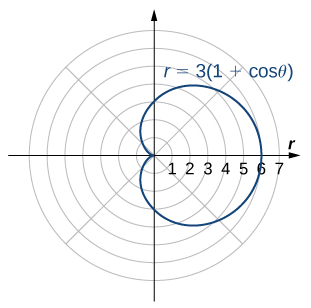
\includegraphics[scale=0.5]{imagens/int19.png}}\\
    \footnotesize{Gilbert Strang \& Edwin Herman: \emph{Calculus}
        (ed.\ online, 2017, vol.\ 2, pg.\ 652)}
  \end{center}
\end{figure}

\begin{figure}[H]
  \begin{center}
    \caption{A beleza polar: Limaçon}
    \label{fig:belo3}
    \fbox{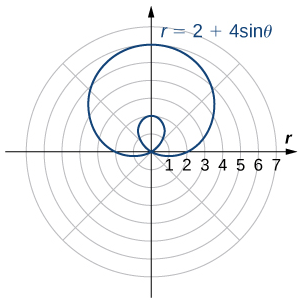
\includegraphics[scale=0.5]{imagens/int20.png}}\\
    \footnotesize{Gilbert Strang \& Edwin Herman: \emph{Calculus}
         (ed.\ online, 2017, vol.\ 2, pg.\ 652)}
  \end{center}
\end{figure}

\begin{figure}[H]
  \begin{center}
    \caption{A beleza polar: rosácea}
    \label{fig:belo4}
    \fbox{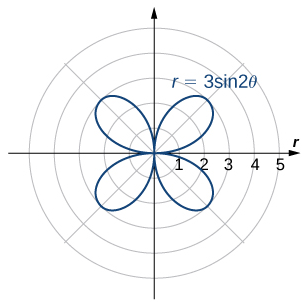
\includegraphics[scale=0.5]{imagens/int21.png}}\\
    \footnotesize{Gilbert Strang \& Edwin Herman: \emph{Calculus}
          (ed.\ online, 2017, vol.\ 2, pg.\ 652)}
  \end{center}
\end{figure}

\begin{figure}[H]
  \begin{center}
    \caption{A beleza polar: rosácea com 3 pétalas}
    \label{fig:belo5}
    \fbox{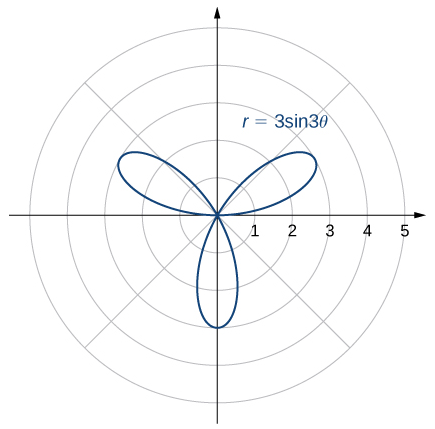
\includegraphics[scale=0.38]{imagens/int22.png}}\\
    \footnotesize{Gilbert Strang \& Edwin Herman: \emph{Calculus}
          (ed.\ online, 2017, vol.\ 2, pg.\ 652)}
  \end{center}
\end{figure}

\begin{figure}[H]
  \begin{center}
    \caption{A beleza polar: formas inusitadas}
    \label{fig:belo6}
    \fbox{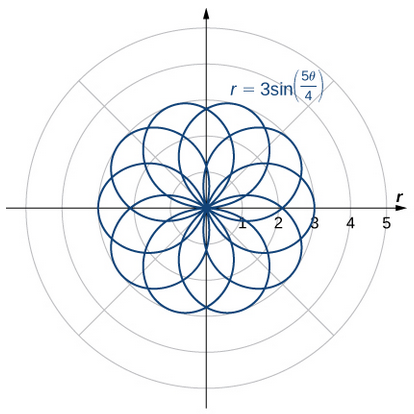
\includegraphics[scale=0.4]{imagens/int23.png}}\\
    \footnotesize{Gilbert Strang \& Edwin Herman: \emph{Calculus}
         (ed.\ online, 2017, vol.\ 2, pg.\ 652)}
  \end{center}
\end{figure}

\begin{figure}[H]
  \begin{center}
    \caption{A beleza polar: espiral logarítmica}
    \label{fig:belo7}
    \fbox{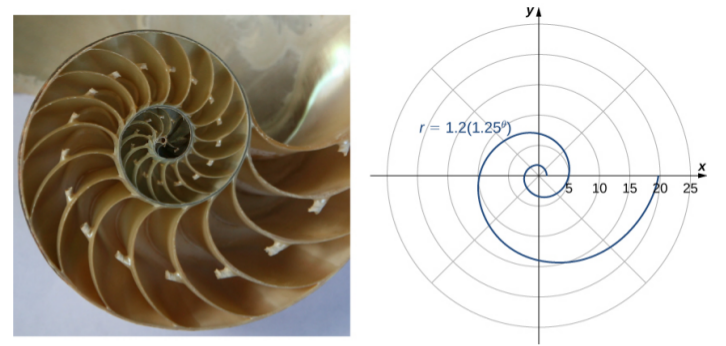
\includegraphics[scale=0.45]{imagens/int24.png}}\\
    \footnotesize{Gilbert Strang \& Edwin Herman: \emph{Calculus}
          (ed.\ online, 2017, vol.\ 2, pg.\ 655)}
  \end{center}
\end{figure}

Não é possível deixar de notar, pela figura~\ref{fig:belo7}, como uma
simples função matemática, $r = 1.2(1.25^\theta)$, pode ser utilizada
para descrever uma obra de Deus, uma obra da criação. Isso nos faz
pensar que Galileu Galilei estava correto ao dizer que ``a matemática
é o alfabeto que Deus usou para escrever o universo''\footnote{Apesar
  de universalmene conhecida e atribuída à Galileu, sabe-se que ele
  não escreveu exatamente isso. Uma simples pesquisa na internet
  mostrará diversas citações semelhantes e polêmicas quanto a versão
  exata ou correta da frase.}.


\subsection{De retangular para polar e vice-versa}
\label{sec:coordpolar-equiv}

Como uma mesma função pode ser expressa tanto em coordenadas
retangulares quanto em coordenadas polares, existe um modo direto de
transformar coordenadas retangulares em polares e vice-versa
(figura~\ref{fig:retpol}) utilizando-se trigonometria:

\begin{figure}[H]
  \begin{center}
    \caption{Retangular $\leftrightarrows$ Polar}
    \label{fig:retpol}
    \fbox{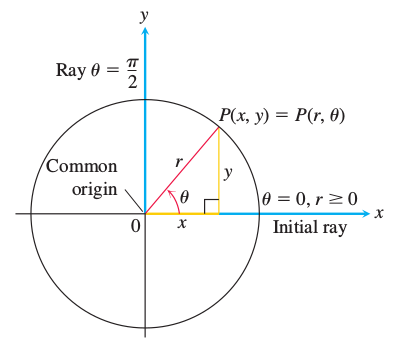
\includegraphics[scale=0.6]{imagens/int25.png}}\\
    \footnotesize{George Thomas: \emph{Thomas' Calculus: early transcedentals}
          (14ª ed., 2017, pg.\ 683)}
  \end{center}
\end{figure}

A transformação de coordenadas polares em coordenadas retangulares
é dada por:

\begin{equation}
  x = r \cos(\theta)
\end{equation}
\begin{equation}
  y = r \sin(\theta)
\end{equation}

E a transformação de coordenadas retangulares em coordenadas polares é
dada por (cuidado para que o sinal de $r$ e a escolha de $\theta$
sejam consistentes com o quadrante no qual o ponto $(x, y)$ está):

\begin{equation}
  r^2 = x^2 + y^2
\end{equation}
\begin{equation}
  \tan(\theta) = \frac{y}{x} \quad \therefore \quad \theta = \arctan\left(\frac{y}{x}\right)
\end{equation}

Essas transformações entre coordenadas retangulares e polares serão
fundamentais para o cálculo do volume utilizando-se integrais.
